\documentclass[10pt]{article}

% --- Page Layout and Columns ---
\usepackage[letterpaper, top=1.125in, bottom=1.125in, left=0.85in, right=0.85in]{geometry}
\usepackage{multicol}
\setlength{\columnsep}{0.25in}  % Set col gap
\setlength{\hsize}{3.275in}     % Set col width

% --- Font and Spacing ---
\usepackage{fontspec}
\usepackage{anyfontsize}
\usepackage{setspace}

\setmainfont{TeX Gyre Termes}

\linespread{1.0} % Keeps base line spacing
\setstretch{1.2} % 10pt font × 1.2 = exactly 12pt line spacing


% --- Paragraph Settings ---
\setlength{\parindent}{0.125in}
\setlength{\parskip}{0pt}

\usepackage{ragged2e}
\justifying

% --- Section and Subsection Formatting ---
\usepackage{titlesec}

% Section: Roman numerals, small caps, centered (e.g., I. INTRODUCTION)
\titleformat{\section}
  {\centering\normalfont\fontsize{10pt}{12pt}\scshape} % 10pt bold, centered
  {\thesection.}{0.5em}{}

\titlespacing*{\section}{0pt}{18pt}{6pt}
\renewcommand{\thesection}{\Roman{section}}

% Subsection: Alphabet labels, italic, indented first paragraph
\titleformat{\subsection}[hang]
  {\normalfont\fontsize{10pt}{12pt}\itshape}
  {\thesubsection.}{0.5em}{}

\titlespacing*{\subsection}{0pt}{6pt}{6pt}
\renewcommand{\thesubsection}{\Alph{subsection}}

\makeatletter
\let\@afterindentfalse\@afterindenttrue
\makeatother

% --- Math and Equation Formatting ---
\usepackage{amsmath}

% Adjust spacing before and after equations (6pt = approx. 0.0833in)
\expandafter\def\expandafter\displaymath@hook\expandafter{%
  \displaymath@hook
  \addtolength{\abovedisplayskip}{-6pt}
  \addtolength{\belowdisplayskip}{-6pt}
}

% --- Figure Formatting ---
\usepackage{hyperref}
\usepackage{graphicx}
\usepackage{caption}
\usepackage{mwe} % for example-image

% IEEE-style figure captions
\captionsetup[figure]{
  font=footnotesize,           % 9pt Times (footnotesize ≈ 9pt)
  justification=justified,     % fully justified
  singlelinecheck=false,       % don't center short captions
  labelsep=period,             % "Fig. 1." instead of colon
  skip=10pt                    % spacing above caption
}

% --- Document Style ---
\pagestyle{empty} % Remove page numbers

% --- Bibliography Formatting ---


% --- Document Start ---
\begin{document}

% --- Start two-column layout ---
\begin{multicols}{2}

% --- Title, authors, and department ---
\begin{center}
    {\fontsize{18pt}{22pt}\selectfont RAPID-X Digital ASIC Tapeout\par}

    \vspace{1em}
    
    \fontsize{12pt}{14pt}{\selectfont Davi Dantas, Evan Kasky, Youssef Samwel, Pablo Rodriguez, Timothy Ogg, Nicolas Sayed\par}

    \vspace{1em}
    
    {\selectfont Dept. of Electrical Engineering and Computer Science, University of Central Florida, Orlando, Florida, 32816-2450\par}
    
\end{center}

% --- Abstract Section ---
{\fontsize{9pt}{10pt}\selectfont
\setlength{\parindent}{0.125in}
\textbf{\textit{Abstract}\ \ --- \ \ Use 9 point Times New Roman Bold font for the abstract. Set your line spacing to be 10 points rather than single space. Indent the first line by 0.125 inches and type the word “Abstract” in 9 point Times New Roman Bold Italic. This should be followed by two spaces, a long dash (option / shift / minus), two spaces, and then the first word of your abstract (as shown above). Please try to keep the length of your abstract to 100 words or less. Times font is an acceptable substitute for Times New Roman font. After the abstract, you should list a few key words from the IEEE approved “Index Terms” LIST that describe your paper. The index terms are used by automated IEEE search engines to quickly locate your paper. Typically, you should list about 5 to 7 key words, in alphabetical order, using 9 point Times New Roman Bold font. An example is shown next.}

\vspace{0pt}

\textbf{ \textit{Index Terms} \ \ --- \ \ Ceramics, coaxial resonators, delay filters, delay-lines, power amplifiers. }

}

% --- INTODUCTION ---
\section{INTRODUCTION}
Lorem ipsum dolor sit amet, consectetur adipiscing elit. Suspendisse vel lorem nec nisi luctus lobortis. Quisque ullamcorper finibus congue. Aliquam id quam neque. Interdum et malesuada fames ac ante ipsum primis in faucibus. Duis laoreet porttitor libero, eget vestibulum sem hendrerit vitae. Nulla pretium ipsum vitae nisl varius, consectetur auctor ante varius. Donec vel purus nec diam tristique blandit sit amet in neque. Vestibulum dapibus, ipsum in varius blandit, diam arcu cursus erat, eu luctus enim mi bibendum mi. Nunc porta tellus viverra laoreet commodo. Mauris mattis lacus vitae lorem eleifend tincidunt. Donec in tellus interdum, auctor risus fermentum, laoreet mi. Curabitur id enim metus. Sed convallis vulputate purus vel faucibus.\cite{cantrell2000}

Suspendisse faucibus rhoncus orci, vel dictum nulla fermentum ut. Praesent ligula velit, malesuada eu quam quis, ornare bibendum sem. Quisque posuere dapibus urna, at eleifend odio venenatis sit amet. Aenean eleifend blandit eleifend. Nulla tincidunt orci est, quis aliquet lorem gravida nec. Duis consectetur vehicula nulla aliquet mollis. Vivamus a finibus massa. Quisque vel lacus cursus, dignissim dui eget, sagittis erat. Proin in viverra tellus. Sed vel rutrum mi, id lobortis libero. Aliquam quis pharetra nulla. Etiam sed purus lacus. Nullam elementum aliquet purus, a luctus justo ultrices eu. Sed consectetur maximus odio et facilisis. Nam viverra, purus ut facilisis dignissim, risus ante laoreet odio, ac sagittis nisl diam consectetur nulla. Integer ultrices risus mauris, eget vehicula dolor varius ut.

\vspace{12pt}

\noindent
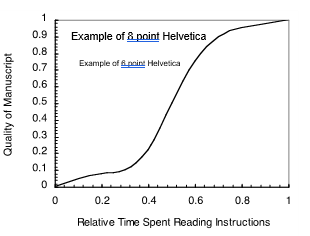
\includegraphics[width=\linewidth]{img.png}

% Create a reference anchor here
\phantomsection
\label{fig:author-time}

\vspace{3pt}

{\fontsize{9pt}{10pt}\selectfont
\noindent\textbf{Fig. 1.} \hspace{0.5in} Estimated relationship between the time an author spends reading these instructions and the quality of the author's digest article.
}

\vspace{12pt}


Sed viverra consequat dignissim. Suspendisse maximus, arcu et porttitor efficitur, nunc leo tempor ante, sed fringilla ante enim quis nulla. Etiam sodales purus tellus, in ullamcorper massa vehicula ut. Aliquam consectetur leo et lectus bibendum sagittis. Morbi non sollicitudin est. Suspendisse iaculis nunc eget enim scelerisque, sed iaculis eros scelerisque. Aliquam erat volutpat. Nulla congue urna nisl, hendrerit porta mauris egestas ut. Integer libero diam, maximus in orci a, pharetra tempus magna.

\subsection{Test Subsection}
Curabitur viverra lectus vitae erat porttitor bibendum. Nam vel elit ut enim dapibus eleifend vitae non quam. Suspendisse a odio non tellus tristique ornare. Suspendisse magna libero, vulputate ac iaculis sit amet, facilisis et risus. Duis eget euismod nisi. Phasellus mollis pulvinar mauris et placerat. Mauris ut condimentum enim. Etiam consequat porttitor nibh vel consectetur. Nulla blandit nunc ut elit venenatis ornare. Ut at orci non purus tempor fermentum. Duis sodales sodales libero, et lacinia felis egestas eget. Phasellus vulputate ipsum nec ullamcorper tincidunt. Nullam consectetur a est id lacinia. Lorem ipsum dolor sit amet, consectetur adipiscing elit.

\begin{equation}
E = mc^2
\end{equation}

Vivamus non sem a leo facilisis tempor sed in quam. Curabitur eget molestie ipsum, id posuere eros. Morbi vestibulum non massa et lobortis. In auctor sapien erat, sed efficitur erat blandit ut. Pellentesque vel rhoncus ex. Nulla vitae rutrum purus. Nulla lacinia eros non iaculis maximus. Aenean laoreet fermentum bibendum. Aliquam sit amet mauris volutpat, pretium lectus quis, venenatis dolor. Vestibulum quis tellus venenatis lectus consequat iaculis vitae fringilla quam. Proin risus nisl, pharetra eu velit non, molestie eleifend turpis.

Phasellus in dictum neque. Aliquam erat volutpat. Nullam bibendum est vitae tellus mattis, sit amet fringilla lectus efficitur. Etiam semper laoreet interdum. Nam placerat massa lacus, in egestas est rhoncus id. Vivamus pulvinar sapien sit amet hendrerit pellentesque. Integer enim lacus, varius vitae neque nec, tristique luctus dolor. Ut non neque justo.

Class aptent taciti sociosqu ad litora torquent per conubia nostra, per inceptos himenaeos. Nulla ut purus nec augue aliquet varius. Morbi cursus erat at arcu rutrum, vel tristique ligula finibus. Integer euismod ligula vel molestie sodales. In ex tellus, finibus sit amet erat sed, consectetur iaculis nisi. Quisque gravida sagittis quam, ac lobortis ipsum blandit id. Donec egestas pulvinar eleifend.

Aliquam non maximus odio. Proin id aliquam lacus. Maecenas quis enim vitae orci euismod rhoncus sit amet vel justo. Vestibulum nibh nunc, suscipit at ante nec, feugiat tristique tortor. Sed vitae est nisi. Donec et ligula urna. Morbi ultrices sem eget mauris dictum mollis. In risus felis, lacinia sed tellus sit amet, lobortis consequat leo. Suspendisse tincidunt eros in scelerisque mollis.

% --- REFERENCES ---
\renewcommand{\refname}{} % Suppress default "References" title
\vspace{12pt}
{\centering\fontsize{10pt}{12pt}\selectfont\scshape REFERENCES\par}
\vspace{-32pt} % Negative space to reduce the gap (This dosen't feel right but i cant get it to work anyway else)

\bibliographystyle{IEEEtran}
\bibliography{references}

\end{multicols}

\end{document}
